\documentclass[1p]{elsarticle_modified}
%\bibliographystyle{elsarticle-num}

%\usepackage[colorlinks]{hyperref}
%\usepackage{abbrmath_seonhwa} %\Abb, \Ascr, \Acal ,\Abf, \Afrak
\usepackage{amsfonts}
\usepackage{amssymb}
\usepackage{amsmath}
\usepackage{amsthm}
\usepackage{scalefnt}
\usepackage{amsbsy}
\usepackage{kotex}
\usepackage{caption}
\usepackage{subfig}
\usepackage{color}
\usepackage{graphicx}
\usepackage{xcolor} %% white, black, red, green, blue, cyan, magenta, yellow
\usepackage{float}
\usepackage{setspace}
\usepackage{hyperref}

\usepackage{tikz}
\usetikzlibrary{arrows}

\usepackage{multirow}
\usepackage{array} % fixed length table
\usepackage{hhline}

%%%%%%%%%%%%%%%%%%%%%
\makeatletter
\renewcommand*\env@matrix[1][\arraystretch]{%
	\edef\arraystretch{#1}%
	\hskip -\arraycolsep
	\let\@ifnextchar\new@ifnextchar
	\array{*\c@MaxMatrixCols c}}
\makeatother %https://tex.stackexchange.com/questions/14071/how-can-i-increase-the-line-spacing-in-a-matrix
%%%%%%%%%%%%%%%

\usepackage[normalem]{ulem}

\newcommand{\msout}[1]{\ifmmode\text{\sout{\ensuremath{#1}}}\else\sout{#1}\fi}
%SOURCE: \msout is \stkout macro in https://tex.stackexchange.com/questions/20609/strikeout-in-math-mode

\newcommand{\cancel}[1]{
	\ifmmode
	{\color{red}\msout{#1}}
	\else
	{\color{red}\sout{#1}}
	\fi
}

\newcommand{\add}[1]{
	{\color{blue}\uwave{#1}}
}

\newcommand{\replace}[2]{
	\ifmmode
	{\color{red}\msout{#1}}{\color{blue}\uwave{#2}}
	\else
	{\color{red}\sout{#1}}{\color{blue}\uwave{#2}}
	\fi
}

\newcommand{\Sol}{\mathcal{S}} %segment
\newcommand{\D}{D} %diagram
\newcommand{\A}{\mathcal{A}} %arc


%%%%%%%%%%%%%%%%%%%%%%%%%%%%%5 test

\def\sl{\operatorname{\textup{SL}}(2,\Cbb)}
\def\psl{\operatorname{\textup{PSL}}(2,\Cbb)}
\def\quan{\mkern 1mu \triangleright \mkern 1mu}

\theoremstyle{definition}
\newtheorem{thm}{Theorem}[section]
\newtheorem{prop}[thm]{Proposition}
\newtheorem{lem}[thm]{Lemma}
\newtheorem{ques}[thm]{Question}
\newtheorem{cor}[thm]{Corollary}
\newtheorem{defn}[thm]{Definition}
\newtheorem{exam}[thm]{Example}
\newtheorem{rmk}[thm]{Remark}
\newtheorem{alg}[thm]{Algorithm}

\newcommand{\I}{\sqrt{-1}}
\begin{document}

%\begin{frontmatter}
%
%\title{Boundary parabolic representations of knots up to 8 crossings}
%
%%% Group authors per affiliation:
%\author{Yunhi Cho} 
%\address{Department of Mathematics, University of Seoul, Seoul, Korea}
%\ead{yhcho@uos.ac.kr}
%
%
%\author{Seonhwa Kim} %\fnref{s_kim}}
%\address{Center for Geometry and Physics, Institute for Basic Science, Pohang, 37673, Korea}
%\ead{ryeona17@ibs.re.kr}
%
%\author{Hyuk Kim}
%\address{Department of Mathematical Sciences, Seoul National University, Seoul 08826, Korea}
%\ead{hyukkim@snu.ac.kr}
%
%\author{Seokbeom Yoon}
%\address{Department of Mathematical Sciences, Seoul National University, Seoul, 08826,  Korea}
%\ead{sbyoon15@snu.ac.kr}
%
%\begin{abstract}
%We find all boundary parabolic representation of knots up to 8 crossings.
%
%\end{abstract}
%\begin{keyword}
%    \MSC[2010] 57M25 
%\end{keyword}
%
%\end{frontmatter}

%\linenumbers
%\tableofcontents
%
\newcommand\colored[1]{\textcolor{white}{\rule[-0.35ex]{0.8em}{1.4ex}}\kern-0.8em\color{red} #1}%
%\newcommand\colored[1]{\textcolor{white}{ #1}\kern-2.17ex	\textcolor{white}{ #1}\kern-1.81ex	\textcolor{white}{ #1}\kern-2.15ex\color{red}#1	}

{\Large $\underline{11a_{216}~(K11a_{216})}$}

\setlength{\tabcolsep}{10pt}
\renewcommand{\arraystretch}{1.6}
\vspace{1cm}\begin{tabular}{m{100pt}>{\centering\arraybackslash}m{274pt}}
\multirow{5}{120pt}{
	\centering
	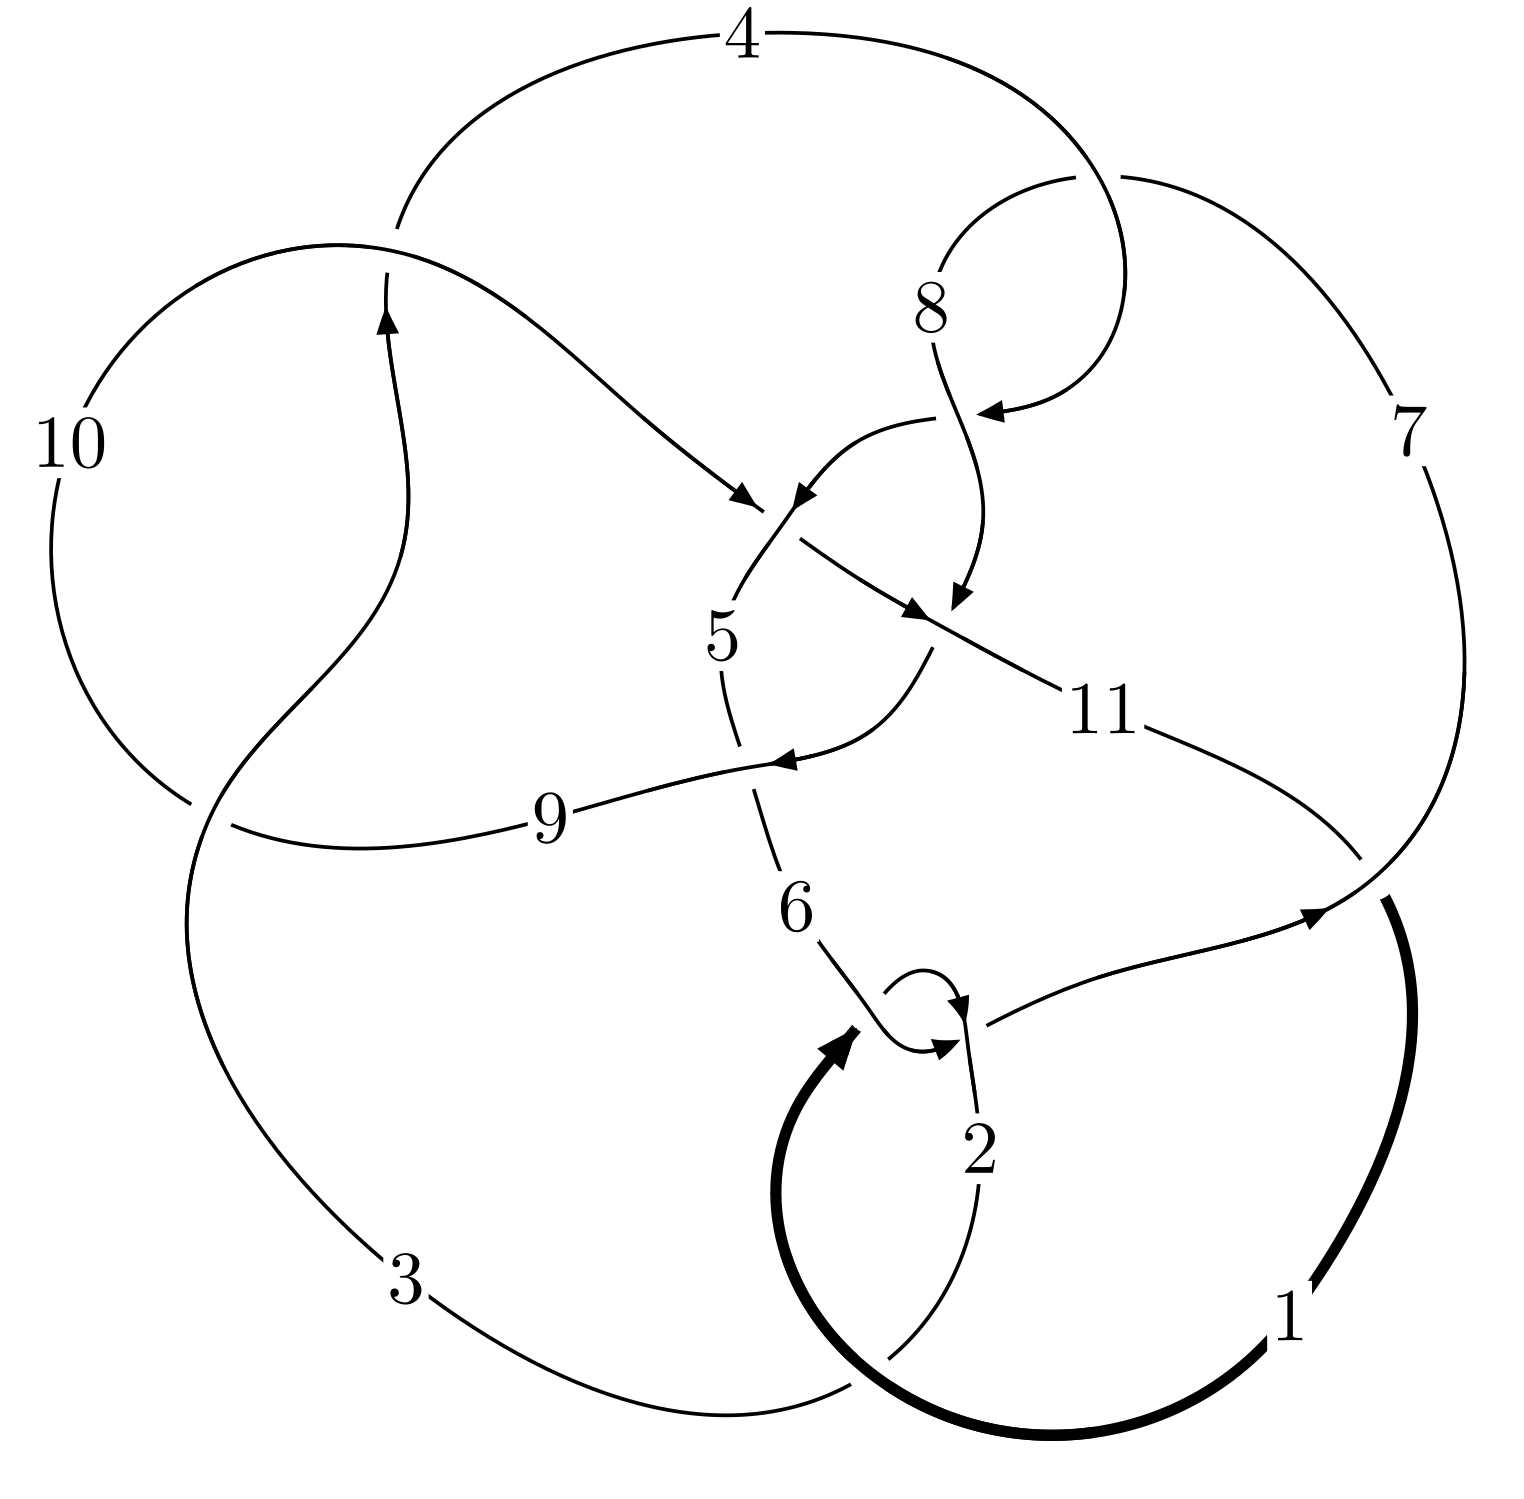
\includegraphics[width=112pt]{../../../GIT/diagram.site/Diagrams/png/465_11a_216.png}\\
\ \ \ A knot diagram\footnotemark}&
\allowdisplaybreaks
\textbf{Linearized knot diagam} \\
\cline{2-2}
 &
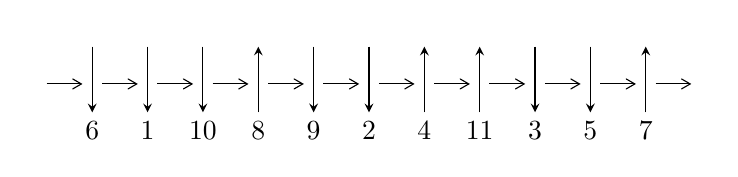
\begin{tikzpicture}[x=20pt, y=17pt]
	% nodes
	\node (C0) at (0, 0) {};
	\node (C1) at (1, 0) {};
	\node (C1U) at (1, +1) {};
	\node (C1D) at (1, -1) {6};

	\node (C2) at (2, 0) {};
	\node (C2U) at (2, +1) {};
	\node (C2D) at (2, -1) {1};

	\node (C3) at (3, 0) {};
	\node (C3U) at (3, +1) {};
	\node (C3D) at (3, -1) {10};

	\node (C4) at (4, 0) {};
	\node (C4U) at (4, +1) {};
	\node (C4D) at (4, -1) {8};

	\node (C5) at (5, 0) {};
	\node (C5U) at (5, +1) {};
	\node (C5D) at (5, -1) {9};

	\node (C6) at (6, 0) {};
	\node (C6U) at (6, +1) {};
	\node (C6D) at (6, -1) {2};

	\node (C7) at (7, 0) {};
	\node (C7U) at (7, +1) {};
	\node (C7D) at (7, -1) {4};

	\node (C8) at (8, 0) {};
	\node (C8U) at (8, +1) {};
	\node (C8D) at (8, -1) {11};

	\node (C9) at (9, 0) {};
	\node (C9U) at (9, +1) {};
	\node (C9D) at (9, -1) {3};

	\node (C10) at (10, 0) {};
	\node (C10U) at (10, +1) {};
	\node (C10D) at (10, -1) {5};

	\node (C11) at (11, 0) {};
	\node (C11U) at (11, +1) {};
	\node (C11D) at (11, -1) {7};
	\node (C12) at (12, 0) {};

	% arrows
	\draw[->,>={angle 60}]
	(C0) edge (C1) (C1) edge (C2) (C2) edge (C3) (C3) edge (C4) (C4) edge (C5) (C5) edge (C6) (C6) edge (C7) (C7) edge (C8) (C8) edge (C9) (C9) edge (C10) (C10) edge (C11) (C11) edge (C12) ;	\draw[->,>=stealth]
	(C1U) edge (C1D) (C2U) edge (C2D) (C3U) edge (C3D) (C4D) edge (C4U) (C5U) edge (C5D) (C6U) edge (C6D) (C7D) edge (C7U) (C8D) edge (C8U) (C9U) edge (C9D) (C10U) edge (C10D) (C11D) edge (C11U) ;
	\end{tikzpicture} \\
\hhline{~~} \\& 
\textbf{Solving Sequence} \\ \cline{2-2} 
 &
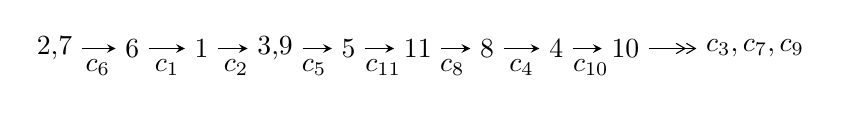
\begin{tikzpicture}[x=25pt, y=7pt]
	% node
	\node (A0) at (-1/8, 0) {2,7};
	\node (A1) at (1, 0) {6};
	\node (A2) at (2, 0) {1};
	\node (A3) at (49/16, 0) {3,9};
	\node (A4) at (33/8, 0) {5};
	\node (A5) at (41/8, 0) {11};
	\node (A6) at (49/8, 0) {8};
	\node (A7) at (57/8, 0) {4};
	\node (A8) at (65/8, 0) {10};
	\node (C1) at (1/2, -1) {$c_{6}$};
	\node (C2) at (3/2, -1) {$c_{1}$};
	\node (C3) at (5/2, -1) {$c_{2}$};
	\node (C4) at (29/8, -1) {$c_{5}$};
	\node (C5) at (37/8, -1) {$c_{11}$};
	\node (C6) at (45/8, -1) {$c_{8}$};
	\node (C7) at (53/8, -1) {$c_{4}$};
	\node (C8) at (61/8, -1) {$c_{10}$};
	\node (A9) at (10, 0) {$c_{3},c_{7},c_{9}$};

	% edge
	\draw[->,>=stealth]	
	(A0) edge (A1) (A1) edge (A2) (A2) edge (A3) (A3) edge (A4) (A4) edge (A5) (A5) edge (A6) (A6) edge (A7) (A7) edge (A8) ;
	\draw[->>,>={angle 60}]	
	(A8) edge (A9);
\end{tikzpicture} \\ 

\end{tabular} \\

\footnotetext{
The image of knot diagram is generated by the software ``\textbf{Draw programme}" developed by Andrew Bartholomew(\url{http://www.layer8.co.uk/maths/draw/index.htm\#Running-draw}), where we modified some parts for our purpose(\url{https://github.com/CATsTAILs/LinksPainter}).
}\phantom \\ \newline 
\centering \textbf{Ideals for irreducible components\footnotemark of $X_{\text{par}}$} 
 
\begin{align*}
I^u_{1}&=\langle 
-1.00850\times10^{59} u^{80}-3.71314\times10^{58} u^{79}+\cdots+1.36235\times10^{58} b-1.35990\times10^{59},\\
\phantom{I^u_{1}}&\phantom{= \langle  }1.76890\times10^{59} u^{80}+8.72974\times10^{58} u^{79}+\cdots+1.36235\times10^{58} a+2.94938\times10^{59},\;u^{81}+u^{80}+\cdots+2 u+1\rangle \\
I^u_{2}&=\langle 
-2 u^{14}+2 u^{13}+7 u^{12}-7 u^{11}-12 u^{10}+12 u^9+9 u^8-7 u^7-4 u^6-3 u^5+3 u^4+6 u^3-5 u^2+b-2 u+3,\\
\phantom{I^u_{2}}&\phantom{= \langle  }-3 u^{13}+u^{12}+10 u^{11}-3 u^{10}-17 u^9+4 u^8+12 u^7+u^6-4 u^5-7 u^4+7 u^2+a-2 u-4,\\
\phantom{I^u_{2}}&\phantom{= \langle  }u^{15}-4 u^{13}+8 u^{11}-8 u^9- u^8+4 u^7+3 u^6-4 u^4+3 u^2-1\rangle \\
I^u_{3}&=\langle 
u^2+b,\;- u^2+a-1,\;u^6+u^5+1\rangle \\
I^u_{4}&=\langle 
b+1,\;a-2,\;u-1\rangle \\
\\
\end{align*}
\raggedright * 4 irreducible components of $\dim_{\mathbb{C}}=0$, with total 103 representations.\\
\footnotetext{All coefficients of polynomials are rational numbers. But the coefficients are sometimes approximated in decimal forms when there is not enough margin.}
\newpage
\renewcommand{\arraystretch}{1}
\centering \section*{I. $I^u_{1}= \langle -1.01\times10^{59} u^{80}-3.71\times10^{58} u^{79}+\cdots+1.36\times10^{58} b-1.36\times10^{59},\;1.77\times10^{59} u^{80}+8.73\times10^{58} u^{79}+\cdots+1.36\times10^{58} a+2.95\times10^{59},\;u^{81}+u^{80}+\cdots+2 u+1 \rangle$}
\flushleft \textbf{(i) Arc colorings}\\
\begin{tabular}{m{7pt} m{180pt} m{7pt} m{180pt} }
\flushright $a_{2}=$&$\begin{pmatrix}0\\u\end{pmatrix}$ \\
\flushright $a_{7}=$&$\begin{pmatrix}1\\0\end{pmatrix}$ \\
\flushright $a_{6}=$&$\begin{pmatrix}1\\- u^2\end{pmatrix}$ \\
\flushright $a_{1}=$&$\begin{pmatrix}u\\- u^3+u\end{pmatrix}$ \\
\flushright $a_{3}=$&$\begin{pmatrix}- u^3\\u^5- u^3+u\end{pmatrix}$ \\
\flushright $a_{9}=$&$\begin{pmatrix}-12.9842 u^{80}-6.40783 u^{79}+\cdots-2.14853 u-21.6491\\7.40264 u^{80}+2.72553 u^{79}+\cdots+4.39790 u+9.98198\end{pmatrix}$ \\
\flushright $a_{5}=$&$\begin{pmatrix}-13.3712 u^{80}-5.09999 u^{79}+\cdots-2.91497 u-20.5076\\0.0913650 u^{80}-0.813439 u^{79}+\cdots-2.45718 u-2.62055\end{pmatrix}$ \\
\flushright $a_{11}=$&$\begin{pmatrix}u^3\\- u^3+u\end{pmatrix}$ \\
\flushright $a_{8}=$&$\begin{pmatrix}-14.4485 u^{80}-7.48009 u^{79}+\cdots-2.78649 u-23.7611\\5.28092 u^{80}+2.32374 u^{79}+\cdots+4.14897 u+5.26440\end{pmatrix}$ \\
\flushright $a_{4}=$&$\begin{pmatrix}-8.40559 u^{80}-5.75051 u^{79}+\cdots+2.69355 u-17.0429\\-6.46426 u^{80}-2.78674 u^{79}+\cdots-6.07564 u-10.4024\end{pmatrix}$ \\
\flushright $a_{10}=$&$\begin{pmatrix}-13.0257 u^{80}-6.50801 u^{79}+\cdots-1.60601 u-20.8812\\6.96235 u^{80}+2.92923 u^{79}+\cdots+6.10527 u+7.49207\end{pmatrix}$\\ \flushright $a_{10}=$&$\begin{pmatrix}-13.0257 u^{80}-6.50801 u^{79}+\cdots-1.60601 u-20.8812\\6.96235 u^{80}+2.92923 u^{79}+\cdots+6.10527 u+7.49207\end{pmatrix}$\\&\end{tabular}
\flushleft \textbf{(ii) Obstruction class $= -1$}\\~\\
\flushleft \textbf{(iii) Cusp Shapes $= 14.5586 u^{80}+7.70676 u^{79}+\cdots-1.69347 u+19.4046$}\\~\\
\newpage\renewcommand{\arraystretch}{1}
\flushleft \textbf{(iv) u-Polynomials at the component}\newline \\
\begin{tabular}{m{50pt}|m{274pt}}
Crossings & \hspace{64pt}u-Polynomials at each crossing \\
\hline $$\begin{aligned}c_{1},c_{6}\end{aligned}$$&$\begin{aligned}
&u^{81}- u^{80}+\cdots+2 u-1
\end{aligned}$\\
\hline $$\begin{aligned}c_{2}\end{aligned}$$&$\begin{aligned}
&u^{81}+43 u^{80}+\cdots+6 u+1
\end{aligned}$\\
\hline $$\begin{aligned}c_{3},c_{9}\end{aligned}$$&$\begin{aligned}
&u^{81}-7 u^{80}+\cdots-1188 u+216
\end{aligned}$\\
\hline $$\begin{aligned}c_{4},c_{7}\end{aligned}$$&$\begin{aligned}
&u^{81}-2 u^{80}+\cdots-77 u+79
\end{aligned}$\\
\hline $$\begin{aligned}c_{5}\end{aligned}$$&$\begin{aligned}
&u^{81}+u^{80}+\cdots-16528 u-1781
\end{aligned}$\\
\hline $$\begin{aligned}c_{8}\end{aligned}$$&$\begin{aligned}
&u^{81}+13 u^{80}+\cdots-34 u+11
\end{aligned}$\\
\hline $$\begin{aligned}c_{10}\end{aligned}$$&$\begin{aligned}
&u^{81}- u^{80}+\cdots+14 u+3
\end{aligned}$\\
\hline $$\begin{aligned}c_{11}\end{aligned}$$&$\begin{aligned}
&u^{81}-3 u^{80}+\cdots+4942 u-1947
\end{aligned}$\\
\hline
\end{tabular}\\~\\
\newpage\renewcommand{\arraystretch}{1}
\flushleft \textbf{(v) Riley Polynomials at the component}\newline \\
\begin{tabular}{m{50pt}|m{274pt}}
Crossings & \hspace{64pt}Riley Polynomials at each crossing \\
\hline $$\begin{aligned}c_{1},c_{6}\end{aligned}$$&$\begin{aligned}
&y^{81}-43 y^{80}+\cdots+6 y-1
\end{aligned}$\\
\hline $$\begin{aligned}c_{2}\end{aligned}$$&$\begin{aligned}
&y^{81}+y^{80}+\cdots+38 y-1
\end{aligned}$\\
\hline $$\begin{aligned}c_{3},c_{9}\end{aligned}$$&$\begin{aligned}
&y^{81}-57 y^{80}+\cdots+1333584 y-46656
\end{aligned}$\\
\hline $$\begin{aligned}c_{4},c_{7}\end{aligned}$$&$\begin{aligned}
&y^{81}-50 y^{80}+\cdots-1813 y-6241
\end{aligned}$\\
\hline $$\begin{aligned}c_{5}\end{aligned}$$&$\begin{aligned}
&y^{81}-27 y^{80}+\cdots+148198452 y-3171961
\end{aligned}$\\
\hline $$\begin{aligned}c_{8}\end{aligned}$$&$\begin{aligned}
&y^{81}-7 y^{80}+\cdots+9032 y-121
\end{aligned}$\\
\hline $$\begin{aligned}c_{10}\end{aligned}$$&$\begin{aligned}
&y^{81}-3 y^{80}+\cdots+232 y-9
\end{aligned}$\\
\hline $$\begin{aligned}c_{11}\end{aligned}$$&$\begin{aligned}
&y^{81}+41 y^{80}+\cdots+38652040 y-3790809
\end{aligned}$\\
\hline
\end{tabular}\\~\\
\newpage\flushleft \textbf{(vi) Complex Volumes and Cusp Shapes}
$$\begin{array}{c|c|c}  
\text{Solutions to }I^u_{1}& \I (\text{vol} + \sqrt{-1}CS) & \text{Cusp shape}\\
 \hline 
\begin{aligned}
u &= \phantom{-}0.353486 + 0.936121 I \\
a &= \phantom{-}0.145670 - 0.210945 I \\
b &= -0.684489 + 0.183324 I\end{aligned}
 & -1.81799 + 2.40695 I & \phantom{-0.000000 } 0 \\ \hline\begin{aligned}
u &= \phantom{-}0.353486 - 0.936121 I \\
a &= \phantom{-}0.145670 + 0.210945 I \\
b &= -0.684489 - 0.183324 I\end{aligned}
 & -1.81799 - 2.40695 I & \phantom{-0.000000 } 0 \\ \hline\begin{aligned}
u &= \phantom{-}0.764070 + 0.573116 I \\
a &= \phantom{-}0.019145 - 0.599281 I \\
b &= \phantom{-}0.294520 + 0.973700 I\end{aligned}
 & -1.65399 - 4.34598 I & \phantom{-0.000000 -}0. + 7.39263 I \\ \hline\begin{aligned}
u &= \phantom{-}0.764070 - 0.573116 I \\
a &= \phantom{-}0.019145 + 0.599281 I \\
b &= \phantom{-}0.294520 - 0.973700 I\end{aligned}
 & -1.65399 + 4.34598 I & \phantom{-0.000000 } 0. - 7.39263 I \\ \hline\begin{aligned}
u &= \phantom{-}0.897471 + 0.585786 I \\
a &= -0.426738 - 0.251752 I \\
b &= \phantom{-}0.378705 - 0.463704 I\end{aligned}
 & \phantom{-}4.21372 - 0.52225 I & \phantom{-0.000000 } 0 \\ \hline\begin{aligned}
u &= \phantom{-}0.897471 - 0.585786 I \\
a &= -0.426738 + 0.251752 I \\
b &= \phantom{-}0.378705 + 0.463704 I\end{aligned}
 & \phantom{-}4.21372 + 0.52225 I & \phantom{-0.000000 } 0 \\ \hline\begin{aligned}
u &= -0.255625 + 0.871069 I \\
a &= -0.322424 + 0.317539 I \\
b &= -1.67729 - 0.85921 I\end{aligned}
 & -0.92282 - 11.98720 I & -2.33004 + 6.68936 I \\ \hline\begin{aligned}
u &= -0.255625 - 0.871069 I \\
a &= -0.322424 - 0.317539 I \\
b &= -1.67729 + 0.85921 I\end{aligned}
 & -0.92282 + 11.98720 I & -2.33004 - 6.68936 I \\ \hline\begin{aligned}
u &= \phantom{-}0.887015 + 0.179085 I \\
a &= \phantom{-}1.247820 + 0.507202 I \\
b &= -0.406240 - 0.514609 I\end{aligned}
 & -1.382340 - 0.196561 I & -8.40096 + 0.94389 I \\ \hline\begin{aligned}
u &= \phantom{-}0.887015 - 0.179085 I \\
a &= \phantom{-}1.247820 - 0.507202 I \\
b &= -0.406240 + 0.514609 I\end{aligned}
 & -1.382340 + 0.196561 I & -8.40096 - 0.94389 I\\
 \hline 
 \end{array}$$\newpage$$\begin{array}{c|c|c}  
\text{Solutions to }I^u_{1}& \I (\text{vol} + \sqrt{-1}CS) & \text{Cusp shape}\\
 \hline 
\begin{aligned}
u &= \phantom{-}0.666327 + 0.609855 I \\
a &= -1.056000 + 0.794212 I \\
b &= \phantom{-}0.120020 - 0.152491 I\end{aligned}
 & \phantom{-}4.88164 - 4.17734 I & \phantom{-}2.92030 + 4.97430 I \\ \hline\begin{aligned}
u &= \phantom{-}0.666327 - 0.609855 I \\
a &= -1.056000 - 0.794212 I \\
b &= \phantom{-}0.120020 + 0.152491 I\end{aligned}
 & \phantom{-}4.88164 + 4.17734 I & \phantom{-}2.92030 - 4.97430 I \\ \hline\begin{aligned}
u &= -0.772892 + 0.442862 I \\
a &= \phantom{-}0.911132 + 0.522504 I \\
b &= -0.563301 - 0.466917 I\end{aligned}
 & \phantom{-}1.33705 + 1.90417 I & \phantom{-}2.60969 - 4.16146 I \\ \hline\begin{aligned}
u &= -0.772892 - 0.442862 I \\
a &= \phantom{-}0.911132 - 0.522504 I \\
b &= -0.563301 + 0.466917 I\end{aligned}
 & \phantom{-}1.33705 - 1.90417 I & \phantom{-}2.60969 + 4.16146 I \\ \hline\begin{aligned}
u &= -0.833248 + 0.735410 I \\
a &= -0.309844 - 0.449602 I \\
b &= -0.203212 + 0.411021 I\end{aligned}
 & \phantom{-}2.49951 + 9.29172 I & \phantom{-0.000000 } 0 \\ \hline\begin{aligned}
u &= -0.833248 - 0.735410 I \\
a &= -0.309844 + 0.449602 I \\
b &= -0.203212 - 0.411021 I\end{aligned}
 & \phantom{-}2.49951 - 9.29172 I & \phantom{-0.000000 } 0 \\ \hline\begin{aligned}
u &= -0.839590 + 0.291084 I \\
a &= -0.45851 + 2.35188 I \\
b &= -0.61804 - 1.59554 I\end{aligned}
 & \phantom{-}0.06939 + 4.39534 I & -6.51221 - 9.24323 I \\ \hline\begin{aligned}
u &= -0.839590 - 0.291084 I \\
a &= -0.45851 - 2.35188 I \\
b &= -0.61804 + 1.59554 I\end{aligned}
 & \phantom{-}0.06939 - 4.39534 I & -6.51221 + 9.24323 I \\ \hline\begin{aligned}
u &= -0.789832 + 0.783125 I \\
a &= -0.465566 + 0.452295 I \\
b &= \phantom{-}0.0687710 - 0.1002050 I\end{aligned}
 & \phantom{-}2.65976 - 3.66135 I & \phantom{-0.000000 } 0 \\ \hline\begin{aligned}
u &= -0.789832 - 0.783125 I \\
a &= -0.465566 - 0.452295 I \\
b &= \phantom{-}0.0687710 + 0.1002050 I\end{aligned}
 & \phantom{-}2.65976 + 3.66135 I & \phantom{-0.000000 } 0\\
 \hline 
 \end{array}$$\newpage$$\begin{array}{c|c|c}  
\text{Solutions to }I^u_{1}& \I (\text{vol} + \sqrt{-1}CS) & \text{Cusp shape}\\
 \hline 
\begin{aligned}
u &= \phantom{-}1.032810 + 0.447989 I \\
a &= \phantom{-}2.83612 - 0.49189 I \\
b &= -1.53996 - 1.53611 I\end{aligned}
 & \phantom{-}0.275846 - 0.630932 I & \phantom{-0.000000 } 0 \\ \hline\begin{aligned}
u &= \phantom{-}1.032810 - 0.447989 I \\
a &= \phantom{-}2.83612 + 0.49189 I \\
b &= -1.53996 + 1.53611 I\end{aligned}
 & \phantom{-}0.275846 + 0.630932 I & \phantom{-0.000000 } 0 \\ \hline\begin{aligned}
u &= -1.111980 + 0.324340 I \\
a &= \phantom{-}1.80235 + 1.20589 I \\
b &= -2.24237 + 0.27267 I\end{aligned}
 & -0.79545 - 2.68846 I & \phantom{-0.000000 } 0 \\ \hline\begin{aligned}
u &= -1.111980 - 0.324340 I \\
a &= \phantom{-}1.80235 - 1.20589 I \\
b &= -2.24237 - 0.27267 I\end{aligned}
 & -0.79545 + 2.68846 I & \phantom{-0.000000 } 0 \\ \hline\begin{aligned}
u &= -0.453414 + 0.691603 I \\
a &= -0.0996573 - 0.0433267 I \\
b &= -0.996987 + 0.338045 I\end{aligned}
 & \phantom{-}2.86402 - 1.12377 I & \phantom{-}1.82611 - 2.82977 I \\ \hline\begin{aligned}
u &= -0.453414 - 0.691603 I \\
a &= -0.0996573 + 0.0433267 I \\
b &= -0.996987 - 0.338045 I\end{aligned}
 & \phantom{-}2.86402 + 1.12377 I & \phantom{-}1.82611 + 2.82977 I \\ \hline\begin{aligned}
u &= \phantom{-}0.231721 + 0.787238 I \\
a &= \phantom{-}0.250689 + 0.388970 I \\
b &= \phantom{-}1.75641 - 0.82207 I\end{aligned}
 & -4.21937 + 5.70269 I & -5.14699 - 5.02778 I \\ \hline\begin{aligned}
u &= \phantom{-}0.231721 - 0.787238 I \\
a &= \phantom{-}0.250689 - 0.388970 I \\
b &= \phantom{-}1.75641 + 0.82207 I\end{aligned}
 & -4.21937 - 5.70269 I & -5.14699 + 5.02778 I \\ \hline\begin{aligned}
u &= -1.065070 + 0.538991 I \\
a &= \phantom{-}1.40242 + 1.59557 I \\
b &= -1.70328 + 0.12611 I\end{aligned}
 & \phantom{-}1.05312 + 5.61889 I & \phantom{-0.000000 } 0 \\ \hline\begin{aligned}
u &= -1.065070 - 0.538991 I \\
a &= \phantom{-}1.40242 - 1.59557 I \\
b &= -1.70328 - 0.12611 I\end{aligned}
 & \phantom{-}1.05312 - 5.61889 I & \phantom{-0.000000 } 0\\
 \hline 
 \end{array}$$\newpage$$\begin{array}{c|c|c}  
\text{Solutions to }I^u_{1}& \I (\text{vol} + \sqrt{-1}CS) & \text{Cusp shape}\\
 \hline 
\begin{aligned}
u &= -1.111370 + 0.438228 I \\
a &= \phantom{-}1.385970 + 0.267580 I \\
b &= -0.64009 + 1.54321 I\end{aligned}
 & -5.57621 + 3.25113 I & \phantom{-0.000000 } 0 \\ \hline\begin{aligned}
u &= -1.111370 - 0.438228 I \\
a &= \phantom{-}1.385970 - 0.267580 I \\
b &= -0.64009 - 1.54321 I\end{aligned}
 & -5.57621 - 3.25113 I & \phantom{-0.000000 } 0 \\ \hline\begin{aligned}
u &= \phantom{-}1.125260 + 0.410648 I \\
a &= -1.34414 + 1.12484 I \\
b &= \phantom{-}1.69461 + 0.27601 I\end{aligned}
 & -3.69078 - 1.82728 I & \phantom{-0.000000 } 0 \\ \hline\begin{aligned}
u &= \phantom{-}1.125260 - 0.410648 I \\
a &= -1.34414 - 1.12484 I \\
b &= \phantom{-}1.69461 - 0.27601 I\end{aligned}
 & -3.69078 + 1.82728 I & \phantom{-0.000000 } 0 \\ \hline\begin{aligned}
u &= -0.447441 + 0.661185 I \\
a &= -0.088570 + 0.150125 I \\
b &= -1.232070 - 0.219872 I\end{aligned}
 & \phantom{-}2.87684 - 0.94366 I & \phantom{-}3.19851 + 0.58211 I \\ \hline\begin{aligned}
u &= -0.447441 - 0.661185 I \\
a &= -0.088570 - 0.150125 I \\
b &= -1.232070 + 0.219872 I\end{aligned}
 & \phantom{-}2.87684 + 0.94366 I & \phantom{-}3.19851 - 0.58211 I \\ \hline\begin{aligned}
u &= -1.065000 + 0.572695 I \\
a &= \phantom{-}0.18457 + 1.55186 I \\
b &= -1.040630 - 0.428971 I\end{aligned}
 & \phantom{-}1.06746 + 6.00583 I & \phantom{-0.000000 } 0 \\ \hline\begin{aligned}
u &= -1.065000 - 0.572695 I \\
a &= \phantom{-}0.18457 - 1.55186 I \\
b &= -1.040630 + 0.428971 I\end{aligned}
 & \phantom{-}1.06746 - 6.00583 I & \phantom{-0.000000 } 0 \\ \hline\begin{aligned}
u &= -1.197790 + 0.191469 I \\
a &= \phantom{-}1.080480 + 0.170748 I \\
b &= -0.489918 + 0.440340 I\end{aligned}
 & -7.30328 + 0.66829 I & \phantom{-0.000000 } 0 \\ \hline\begin{aligned}
u &= -1.197790 - 0.191469 I \\
a &= \phantom{-}1.080480 - 0.170748 I \\
b &= -0.489918 - 0.440340 I\end{aligned}
 & -7.30328 - 0.66829 I & \phantom{-0.000000 } 0\\
 \hline 
 \end{array}$$\newpage$$\begin{array}{c|c|c}  
\text{Solutions to }I^u_{1}& \I (\text{vol} + \sqrt{-1}CS) & \text{Cusp shape}\\
 \hline 
\begin{aligned}
u &= \phantom{-}1.120360 + 0.467251 I \\
a &= \phantom{-}1.24527 - 1.30896 I \\
b &= -1.96104 + 0.66304 I\end{aligned}
 & -5.35302 - 4.32976 I & \phantom{-0.000000 } 0 \\ \hline\begin{aligned}
u &= \phantom{-}1.120360 - 0.467251 I \\
a &= \phantom{-}1.24527 + 1.30896 I \\
b &= -1.96104 - 0.66304 I\end{aligned}
 & -5.35302 + 4.32976 I & \phantom{-0.000000 } 0 \\ \hline\begin{aligned}
u &= \phantom{-}1.115380 + 0.480964 I \\
a &= -0.90946 - 1.83248 I \\
b &= -0.309442 + 0.841468 I\end{aligned}
 & -1.19632 - 7.51167 I & \phantom{-0.000000 } 0 \\ \hline\begin{aligned}
u &= \phantom{-}1.115380 - 0.480964 I \\
a &= -0.90946 + 1.83248 I \\
b &= -0.309442 - 0.841468 I\end{aligned}
 & -1.19632 + 7.51167 I & \phantom{-0.000000 } 0 \\ \hline\begin{aligned}
u &= \phantom{-}0.268475 + 0.723594 I \\
a &= -1.083920 - 0.186754 I \\
b &= -1.39346 + 0.97561 I\end{aligned}
 & \phantom{-}3.18792 + 5.71030 I & \phantom{-}0.53106 - 5.73349 I \\ \hline\begin{aligned}
u &= \phantom{-}0.268475 - 0.723594 I \\
a &= -1.083920 + 0.186754 I \\
b &= -1.39346 - 0.97561 I\end{aligned}
 & \phantom{-}3.18792 - 5.71030 I & \phantom{-}0.53106 + 5.73349 I \\ \hline\begin{aligned}
u &= -1.188380 + 0.311281 I \\
a &= -1.75719 - 1.47102 I \\
b &= \phantom{-}1.79283 - 0.05490 I\end{aligned}
 & -8.54999 - 2.22876 I & \phantom{-0.000000 } 0 \\ \hline\begin{aligned}
u &= -1.188380 - 0.311281 I \\
a &= -1.75719 + 1.47102 I \\
b &= \phantom{-}1.79283 + 0.05490 I\end{aligned}
 & -8.54999 + 2.22876 I & \phantom{-0.000000 } 0 \\ \hline\begin{aligned}
u &= -1.137500 + 0.475476 I \\
a &= -2.17624 - 0.33439 I \\
b &= \phantom{-}1.72783 - 1.32004 I\end{aligned}
 & -3.22394 + 6.00881 I & \phantom{-0.000000 } 0 \\ \hline\begin{aligned}
u &= -1.137500 - 0.475476 I \\
a &= -2.17624 + 0.33439 I \\
b &= \phantom{-}1.72783 + 1.32004 I\end{aligned}
 & -3.22394 - 6.00881 I & \phantom{-0.000000 } 0\\
 \hline 
 \end{array}$$\newpage$$\begin{array}{c|c|c}  
\text{Solutions to }I^u_{1}& \I (\text{vol} + \sqrt{-1}CS) & \text{Cusp shape}\\
 \hline 
\begin{aligned}
u &= -0.078476 + 0.744812 I \\
a &= \phantom{-}0.704380 - 0.993703 I \\
b &= \phantom{-}1.305590 - 0.047937 I\end{aligned}
 & -2.16071 - 3.34222 I & -4.83017 + 7.08778 I \\ \hline\begin{aligned}
u &= -0.078476 - 0.744812 I \\
a &= \phantom{-}0.704380 + 0.993703 I \\
b &= \phantom{-}1.305590 + 0.047937 I\end{aligned}
 & -2.16071 + 3.34222 I & -4.83017 - 7.08778 I \\ \hline\begin{aligned}
u &= \phantom{-}1.137170 + 0.533166 I \\
a &= \phantom{-}2.28675 - 0.59226 I \\
b &= -2.03696 - 1.61104 I\end{aligned}
 & \phantom{-}0.65865 - 10.48350 I & \phantom{-0.000000 } 0 \\ \hline\begin{aligned}
u &= \phantom{-}1.137170 - 0.533166 I \\
a &= \phantom{-}2.28675 + 0.59226 I \\
b &= -2.03696 + 1.61104 I\end{aligned}
 & \phantom{-}0.65865 + 10.48350 I & \phantom{-0.000000 } 0 \\ \hline\begin{aligned}
u &= \phantom{-}1.186600 + 0.412439 I \\
a &= -1.40354 + 0.43387 I \\
b &= \phantom{-}1.19145 + 1.27355 I\end{aligned}
 & -5.80693 - 0.69674 I & \phantom{-0.000000 } 0 \\ \hline\begin{aligned}
u &= \phantom{-}1.186600 - 0.412439 I \\
a &= -1.40354 - 0.43387 I \\
b &= \phantom{-}1.19145 - 1.27355 I\end{aligned}
 & -5.80693 + 0.69674 I & \phantom{-0.000000 } 0 \\ \hline\begin{aligned}
u &= -1.178410 + 0.480916 I \\
a &= -1.70444 - 1.06176 I \\
b &= \phantom{-}2.40022 - 0.13432 I\end{aligned}
 & -5.32246 + 7.84641 I & \phantom{-0.000000 } 0 \\ \hline\begin{aligned}
u &= -1.178410 - 0.480916 I \\
a &= -1.70444 + 1.06176 I \\
b &= \phantom{-}2.40022 + 0.13432 I\end{aligned}
 & -5.32246 - 7.84641 I & \phantom{-0.000000 } 0 \\ \hline\begin{aligned}
u &= \phantom{-}1.251330 + 0.270280 I \\
a &= \phantom{-}1.54437 - 1.19181 I \\
b &= -1.72788 + 0.01203 I\end{aligned}
 & -5.81796 + 8.31263 I & \phantom{-0.000000 } 0 \\ \hline\begin{aligned}
u &= \phantom{-}1.251330 - 0.270280 I \\
a &= \phantom{-}1.54437 + 1.19181 I \\
b &= -1.72788 - 0.01203 I\end{aligned}
 & -5.81796 - 8.31263 I & \phantom{-0.000000 } 0\\
 \hline 
 \end{array}$$\newpage$$\begin{array}{c|c|c}  
\text{Solutions to }I^u_{1}& \I (\text{vol} + \sqrt{-1}CS) & \text{Cusp shape}\\
 \hline 
\begin{aligned}
u &= \phantom{-}1.163560 + 0.542163 I \\
a &= -2.49355 + 1.01995 I \\
b &= \phantom{-}2.30668 + 1.00700 I\end{aligned}
 & -6.95659 - 10.65130 I & \phantom{-0.000000 } 0 \\ \hline\begin{aligned}
u &= \phantom{-}1.163560 - 0.542163 I \\
a &= -2.49355 - 1.01995 I \\
b &= \phantom{-}2.30668 - 1.00700 I\end{aligned}
 & -6.95659 + 10.65130 I & \phantom{-0.000000 } 0 \\ \hline\begin{aligned}
u &= -0.686699 + 0.054430 I \\
a &= \phantom{-}1.53780 + 0.66922 I \\
b &= -0.66950 - 1.40480 I\end{aligned}
 & \phantom{-}0.82340 + 2.75519 I & -4.46449 - 1.61172 I \\ \hline\begin{aligned}
u &= -0.686699 - 0.054430 I \\
a &= \phantom{-}1.53780 - 0.66922 I \\
b &= -0.66950 + 1.40480 I\end{aligned}
 & \phantom{-}0.82340 - 2.75519 I & -4.46449 + 1.61172 I \\ \hline\begin{aligned}
u &= -1.186750 + 0.572166 I \\
a &= \phantom{-}2.24475 + 0.84767 I \\
b &= -2.15764 + 1.11820 I\end{aligned}
 & -3.7190 + 17.2795 I & \phantom{-0.000000 } 0 \\ \hline\begin{aligned}
u &= -1.186750 - 0.572166 I \\
a &= \phantom{-}2.24475 - 0.84767 I \\
b &= -2.15764 - 1.11820 I\end{aligned}
 & -3.7190 - 17.2795 I & \phantom{-0.000000 } 0 \\ \hline\begin{aligned}
u &= \phantom{-}1.288520 + 0.326107 I \\
a &= -0.977917 + 0.363557 I \\
b &= \phantom{-}0.859230 + 0.498217 I\end{aligned}
 & -6.39093 - 4.34959 I & \phantom{-0.000000 } 0 \\ \hline\begin{aligned}
u &= \phantom{-}1.288520 - 0.326107 I \\
a &= -0.977917 - 0.363557 I \\
b &= \phantom{-}0.859230 - 0.498217 I\end{aligned}
 & -6.39093 + 4.34959 I & \phantom{-0.000000 } 0 \\ \hline\begin{aligned}
u &= \phantom{-}1.186810 + 0.605790 I \\
a &= \phantom{-}1.066820 - 0.511590 I \\
b &= -1.075190 - 0.313808 I\end{aligned}
 & -4.42307 - 8.03198 I & \phantom{-0.000000 } 0 \\ \hline\begin{aligned}
u &= \phantom{-}1.186810 - 0.605790 I \\
a &= \phantom{-}1.066820 + 0.511590 I \\
b &= -1.075190 + 0.313808 I\end{aligned}
 & -4.42307 + 8.03198 I & \phantom{-0.000000 } 0\\
 \hline 
 \end{array}$$\newpage$$\begin{array}{c|c|c}  
\text{Solutions to }I^u_{1}& \I (\text{vol} + \sqrt{-1}CS) & \text{Cusp shape}\\
 \hline 
\begin{aligned}
u &= -1.230620 + 0.525995 I \\
a &= -1.38150 - 0.39729 I \\
b &= \phantom{-}1.41856 - 0.61959 I\end{aligned}
 & -5.01528 + 5.22835 I & \phantom{-0.000000 } 0 \\ \hline\begin{aligned}
u &= -1.230620 - 0.525995 I \\
a &= -1.38150 + 0.39729 I \\
b &= \phantom{-}1.41856 + 0.61959 I\end{aligned}
 & -5.01528 - 5.22835 I & \phantom{-0.000000 } 0 \\ \hline\begin{aligned}
u &= -0.122761 + 0.636850 I \\
a &= \phantom{-}0.773920 - 0.056125 I \\
b &= \phantom{-}0.994606 + 0.698230 I\end{aligned}
 & -0.40315 - 1.75468 I & -2.66947 + 3.58305 I \\ \hline\begin{aligned}
u &= -0.122761 - 0.636850 I \\
a &= \phantom{-}0.773920 + 0.056125 I \\
b &= \phantom{-}0.994606 - 0.698230 I\end{aligned}
 & -0.40315 + 1.75468 I & -2.66947 - 3.58305 I \\ \hline\begin{aligned}
u &= \phantom{-}0.491013 + 0.385970 I \\
a &= -1.318490 + 0.085313 I \\
b &= -0.86028 + 1.57846 I\end{aligned}
 & \phantom{-}1.91014 - 3.07747 I & \phantom{-}3.39105 + 3.81953 I \\ \hline\begin{aligned}
u &= \phantom{-}0.491013 - 0.385970 I \\
a &= -1.318490 - 0.085313 I \\
b &= -0.86028 - 1.57846 I\end{aligned}
 & \phantom{-}1.91014 + 3.07747 I & \phantom{-}3.39105 - 3.81953 I \\ \hline\begin{aligned}
u &= \phantom{-}0.180434 + 0.529501 I \\
a &= -0.662704 + 1.127170 I \\
b &= -0.591412 - 1.215950 I\end{aligned}
 & \phantom{-}1.34431 + 3.37389 I & -0.27532 - 5.21535 I \\ \hline\begin{aligned}
u &= \phantom{-}0.180434 - 0.529501 I \\
a &= -0.662704 - 1.127170 I \\
b &= -0.591412 + 1.215950 I\end{aligned}
 & \phantom{-}1.34431 - 3.37389 I & -0.27532 + 5.21535 I \\ \hline\begin{aligned}
u &= \phantom{-}0.144994 + 0.507790 I \\
a &= \phantom{-}0.36150 - 2.09518 I \\
b &= -0.958492 - 0.271503 I\end{aligned}
 & -2.71152 + 0.29912 I & -4.85977 + 1.99528 I \\ \hline\begin{aligned}
u &= \phantom{-}0.144994 - 0.507790 I \\
a &= \phantom{-}0.36150 + 2.09518 I \\
b &= -0.958492 + 0.271503 I\end{aligned}
 & -2.71152 - 0.29912 I & -4.85977 - 1.99528 I\\
 \hline 
 \end{array}$$\newpage$$\begin{array}{c|c|c}  
\text{Solutions to }I^u_{1}& \I (\text{vol} + \sqrt{-1}CS) & \text{Cusp shape}\\
 \hline 
\begin{aligned}
u &= -0.479949\phantom{ +0.000000I} \\
a &= -4.18306\phantom{ +0.000000I} \\
b &= -0.0617552\phantom{ +0.000000I}\end{aligned}
 & -2.92420\phantom{ +0.000000I} & \phantom{-}0.818700\phantom{ +0.000000I}\\
 \hline 
 \end{array}$$\newpage\newpage\renewcommand{\arraystretch}{1}
\centering \section*{II. $I^u_{2}= \langle -2 u^{14}+2 u^{13}+\cdots+b+3,\;-3 u^{13}+u^{12}+\cdots+a-4,\;u^{15}-4 u^{13}+\cdots+3 u^2-1 \rangle$}
\flushleft \textbf{(i) Arc colorings}\\
\begin{tabular}{m{7pt} m{180pt} m{7pt} m{180pt} }
\flushright $a_{2}=$&$\begin{pmatrix}0\\u\end{pmatrix}$ \\
\flushright $a_{7}=$&$\begin{pmatrix}1\\0\end{pmatrix}$ \\
\flushright $a_{6}=$&$\begin{pmatrix}1\\- u^2\end{pmatrix}$ \\
\flushright $a_{1}=$&$\begin{pmatrix}u\\- u^3+u\end{pmatrix}$ \\
\flushright $a_{3}=$&$\begin{pmatrix}- u^3\\u^5- u^3+u\end{pmatrix}$ \\
\flushright $a_{9}=$&$\begin{pmatrix}3 u^{13}- u^{12}+\cdots+2 u+4\\2 u^{14}-2 u^{13}+\cdots+2 u-3\end{pmatrix}$ \\
\flushright $a_{5}=$&$\begin{pmatrix}- u^{14}-2 u^{13}+\cdots- u-3\\u^{14}- u^{13}-3 u^{12}+2 u^{11}+5 u^{10}-2 u^9-3 u^8-2 u^7+2 u^6+3 u^5-3 u^3+1\end{pmatrix}$ \\
\flushright $a_{11}=$&$\begin{pmatrix}u^3\\- u^3+u\end{pmatrix}$ \\
\flushright $a_{8}=$&$\begin{pmatrix}3 u^{13}- u^{12}+\cdots+2 u+5\\2 u^{14}- u^{13}+\cdots+2 u-2\end{pmatrix}$ \\
\flushright $a_{4}=$&$\begin{pmatrix}-2 u^{14}-2 u^{13}+\cdots-3 u-4\\u^{12}-3 u^{10}+4 u^8- u^6- u^5- u^4+2 u^3- u+1\end{pmatrix}$ \\
\flushright $a_{10}=$&$\begin{pmatrix}2 u^{13}- u^{12}+\cdots+2 u+3\\2 u^{14}- u^{13}+\cdots+3 u-2\end{pmatrix}$\\ \flushright $a_{10}=$&$\begin{pmatrix}2 u^{13}- u^{12}+\cdots+2 u+3\\2 u^{14}- u^{13}+\cdots+3 u-2\end{pmatrix}$\\&\end{tabular}
\flushleft \textbf{(ii) Obstruction class $= 1$}\\~\\
\flushleft \textbf{(iii) Cusp Shapes $= u^{14}-11 u^{13}-3 u^{12}+43 u^{11}+5 u^{10}-78 u^9-4 u^8+61 u^7+13 u^6-11 u^5-31 u^4-13 u^3+35 u^2-3 u-22$}\\~\\
\newpage\renewcommand{\arraystretch}{1}
\flushleft \textbf{(iv) u-Polynomials at the component}\newline \\
\begin{tabular}{m{50pt}|m{274pt}}
Crossings & \hspace{64pt}u-Polynomials at each crossing \\
\hline $$\begin{aligned}c_{1}\end{aligned}$$&$\begin{aligned}
&u^{15}-4 u^{13}+8 u^{11}-8 u^9+u^8+4 u^7-3 u^6+4 u^4-3 u^2+1
\end{aligned}$\\
\hline $$\begin{aligned}c_{2}\end{aligned}$$&$\begin{aligned}
&u^{15}+8 u^{14}+\cdots+6 u+1
\end{aligned}$\\
\hline $$\begin{aligned}c_{3}\end{aligned}$$&$\begin{aligned}
&u^{15}- u^{14}+\cdots- u+1
\end{aligned}$\\
\hline $$\begin{aligned}c_{4}\end{aligned}$$&$\begin{aligned}
&u^{15}- u^{14}+\cdots- u+1
\end{aligned}$\\
\hline $$\begin{aligned}c_{5}\end{aligned}$$&$\begin{aligned}
&u^{15}+2 u^{13}+u^{12}+3 u^{11}+u^{10}+2 u^9+u^7-2 u^6-3 u^5-4 u^4-1
\end{aligned}$\\
\hline $$\begin{aligned}c_{6}\end{aligned}$$&$\begin{aligned}
&u^{15}-4 u^{13}+8 u^{11}-8 u^9- u^8+4 u^7+3 u^6-4 u^4+3 u^2-1
\end{aligned}$\\
\hline $$\begin{aligned}c_{7}\end{aligned}$$&$\begin{aligned}
&u^{15}+u^{14}+\cdots- u-1
\end{aligned}$\\
\hline $$\begin{aligned}c_{8}\end{aligned}$$&$\begin{aligned}
&u^{15}-2 u^{13}+\cdots-4 u-1
\end{aligned}$\\
\hline $$\begin{aligned}c_{9}\end{aligned}$$&$\begin{aligned}
&u^{15}+u^{14}+\cdots- u-1
\end{aligned}$\\
\hline $$\begin{aligned}c_{10}\end{aligned}$$&$\begin{aligned}
&u^{15}+4 u^{11}+3 u^{10}+2 u^9- u^8-2 u^6- u^5-3 u^4- u^3-2 u^2-1
\end{aligned}$\\
\hline $$\begin{aligned}c_{11}\end{aligned}$$&$\begin{aligned}
&u^{15}+4 u^{13}+\cdots-6 u^2+1
\end{aligned}$\\
\hline
\end{tabular}\\~\\
\newpage\renewcommand{\arraystretch}{1}
\flushleft \textbf{(v) Riley Polynomials at the component}\newline \\
\begin{tabular}{m{50pt}|m{274pt}}
Crossings & \hspace{64pt}Riley Polynomials at each crossing \\
\hline $$\begin{aligned}c_{1},c_{6}\end{aligned}$$&$\begin{aligned}
&y^{15}-8 y^{14}+\cdots+6 y-1
\end{aligned}$\\
\hline $$\begin{aligned}c_{2}\end{aligned}$$&$\begin{aligned}
&y^{15}+16 y^{13}+\cdots+2 y-1
\end{aligned}$\\
\hline $$\begin{aligned}c_{3},c_{9}\end{aligned}$$&$\begin{aligned}
&y^{15}-15 y^{14}+\cdots+11 y-1
\end{aligned}$\\
\hline $$\begin{aligned}c_{4},c_{7}\end{aligned}$$&$\begin{aligned}
&y^{15}-11 y^{14}+\cdots+15 y-1
\end{aligned}$\\
\hline $$\begin{aligned}c_{5}\end{aligned}$$&$\begin{aligned}
&y^{15}+4 y^{14}+\cdots-8 y^2-1
\end{aligned}$\\
\hline $$\begin{aligned}c_{8}\end{aligned}$$&$\begin{aligned}
&y^{15}-4 y^{14}+\cdots+4 y-1
\end{aligned}$\\
\hline $$\begin{aligned}c_{10}\end{aligned}$$&$\begin{aligned}
&y^{15}+8 y^{13}+\cdots-4 y-1
\end{aligned}$\\
\hline $$\begin{aligned}c_{11}\end{aligned}$$&$\begin{aligned}
&y^{15}+8 y^{14}+\cdots+12 y-1
\end{aligned}$\\
\hline
\end{tabular}\\~\\
\newpage\flushleft \textbf{(vi) Complex Volumes and Cusp Shapes}
$$\begin{array}{c|c|c}  
\text{Solutions to }I^u_{2}& \I (\text{vol} + \sqrt{-1}CS) & \text{Cusp shape}\\
 \hline 
\begin{aligned}
u &= -0.997247 + 0.392970 I \\
a &= \phantom{-}2.71489 - 0.62809 I \\
b &= -1.29145 + 1.40184 I\end{aligned}
 & -0.044369 - 0.633415 I & -1.08788 + 2.48026 I \\ \hline\begin{aligned}
u &= -0.997247 - 0.392970 I \\
a &= \phantom{-}2.71489 + 0.62809 I \\
b &= -1.29145 - 1.40184 I\end{aligned}
 & -0.044369 + 0.633415 I & -1.08788 - 2.48026 I \\ \hline\begin{aligned}
u &= -0.221545 + 0.858385 I \\
a &= -0.066551 - 0.561702 I \\
b &= \phantom{-}0.651943 - 0.003032 I\end{aligned}
 & -1.82195 - 1.76571 I & -4.04745 - 0.75169 I \\ \hline\begin{aligned}
u &= -0.221545 - 0.858385 I \\
a &= -0.066551 + 0.561702 I \\
b &= \phantom{-}0.651943 + 0.003032 I\end{aligned}
 & -1.82195 + 1.76571 I & -4.04745 + 0.75169 I \\ \hline\begin{aligned}
u &= \phantom{-}0.589578 + 0.609250 I \\
a &= \phantom{-}0.026910 - 0.340226 I \\
b &= -0.852572 - 0.777911 I\end{aligned}
 & \phantom{-}2.48631 + 2.07411 I & -0.45705 - 2.34926 I \\ \hline\begin{aligned}
u &= \phantom{-}0.589578 - 0.609250 I \\
a &= \phantom{-}0.026910 + 0.340226 I \\
b &= -0.852572 + 0.777911 I\end{aligned}
 & \phantom{-}2.48631 - 2.07411 I & -0.45705 + 2.34926 I \\ \hline\begin{aligned}
u &= \phantom{-}1.030730 + 0.548115 I \\
a &= -0.26464 - 1.93296 I \\
b &= -1.17743 + 0.81712 I\end{aligned}
 & \phantom{-}1.09684 - 6.66891 I & -2.05979 + 11.69980 I \\ \hline\begin{aligned}
u &= \phantom{-}1.030730 - 0.548115 I \\
a &= -0.26464 + 1.93296 I \\
b &= -1.17743 - 0.81712 I\end{aligned}
 & \phantom{-}1.09684 + 6.66891 I & -2.05979 - 11.69980 I \\ \hline\begin{aligned}
u &= -0.734119 + 0.278311 I \\
a &= \phantom{-}0.018935 + 1.247810 I \\
b &= -0.75789 - 1.70123 I\end{aligned}
 & \phantom{-}1.01287 + 3.62441 I & -1.97748 - 8.82225 I \\ \hline\begin{aligned}
u &= -0.734119 - 0.278311 I \\
a &= \phantom{-}0.018935 - 1.247810 I \\
b &= -0.75789 + 1.70123 I\end{aligned}
 & \phantom{-}1.01287 - 3.62441 I & -1.97748 + 8.82225 I\\
 \hline 
 \end{array}$$\newpage$$\begin{array}{c|c|c}  
\text{Solutions to }I^u_{2}& \I (\text{vol} + \sqrt{-1}CS) & \text{Cusp shape}\\
 \hline 
\begin{aligned}
u &= \phantom{-}1.162560 + 0.361615 I \\
a &= -1.017670 + 0.054285 I \\
b &= \phantom{-}0.415367 + 1.176280 I\end{aligned}
 & -6.03108 - 1.76748 I & -8.58457 + 2.09679 I \\ \hline\begin{aligned}
u &= \phantom{-}1.162560 - 0.361615 I \\
a &= -1.017670 - 0.054285 I \\
b &= \phantom{-}0.415367 - 1.176280 I\end{aligned}
 & -6.03108 + 1.76748 I & -8.58457 - 2.09679 I \\ \hline\begin{aligned}
u &= \phantom{-}0.729970\phantom{ +0.000000I} \\
a &= \phantom{-}3.59045\phantom{ +0.000000I} \\
b &= -0.927345\phantom{ +0.000000I}\end{aligned}
 & -3.42072\phantom{ +0.000000I} & -16.5640\phantom{ +0.000000I} \\ \hline\begin{aligned}
u &= -1.194930 + 0.516966 I \\
a &= -1.207100 - 0.512386 I \\
b &= \phantom{-}1.47569 - 0.21174 I\end{aligned}
 & -4.85785 + 6.78722 I & -6.00355 - 4.69104 I \\ \hline\begin{aligned}
u &= -1.194930 - 0.516966 I \\
a &= -1.207100 + 0.512386 I \\
b &= \phantom{-}1.47569 + 0.21174 I\end{aligned}
 & -4.85785 - 6.78722 I & -6.00355 + 4.69104 I\\
 \hline 
 \end{array}$$\newpage\newpage\renewcommand{\arraystretch}{1}
\centering \section*{III. $I^u_{3}= \langle u^2+b,\;- u^2+a-1,\;u^6+u^5+1 \rangle$}
\flushleft \textbf{(i) Arc colorings}\\
\begin{tabular}{m{7pt} m{180pt} m{7pt} m{180pt} }
\flushright $a_{2}=$&$\begin{pmatrix}0\\u\end{pmatrix}$ \\
\flushright $a_{7}=$&$\begin{pmatrix}1\\0\end{pmatrix}$ \\
\flushright $a_{6}=$&$\begin{pmatrix}1\\- u^2\end{pmatrix}$ \\
\flushright $a_{1}=$&$\begin{pmatrix}u\\- u^3+u\end{pmatrix}$ \\
\flushright $a_{3}=$&$\begin{pmatrix}- u^3\\u^5- u^3+u\end{pmatrix}$ \\
\flushright $a_{9}=$&$\begin{pmatrix}u^2+1\\- u^2\end{pmatrix}$ \\
\flushright $a_{5}=$&$\begin{pmatrix}u^5- u^4+2\\- u^5- u^2-1\end{pmatrix}$ \\
\flushright $a_{11}=$&$\begin{pmatrix}u^3\\- u^3+u\end{pmatrix}$ \\
\flushright $a_{8}=$&$\begin{pmatrix}u^4+u^2+1\\- u^4\end{pmatrix}$ \\
\flushright $a_{4}=$&$\begin{pmatrix}u^2+1\\- u^2\end{pmatrix}$ \\
\flushright $a_{10}=$&$\begin{pmatrix}- u^3+u^2+1\\u^5- u^3- u^2+u\end{pmatrix}$\\ \flushright $a_{10}=$&$\begin{pmatrix}- u^3+u^2+1\\u^5- u^3- u^2+u\end{pmatrix}$\\&\end{tabular}
\flushleft \textbf{(ii) Obstruction class $= -1$}\\~\\
\flushleft \textbf{(iii) Cusp Shapes $= -6$}\\~\\
\newpage\renewcommand{\arraystretch}{1}
\flushleft \textbf{(iv) u-Polynomials at the component}\newline \\
\begin{tabular}{m{50pt}|m{274pt}}
Crossings & \hspace{64pt}u-Polynomials at each crossing \\
\hline $$\begin{aligned}c_{1},c_{6},c_{8}\end{aligned}$$&$\begin{aligned}
&u^6- u^5+1
\end{aligned}$\\
\hline $$\begin{aligned}c_{2},c_{4},c_{7}\end{aligned}$$&$\begin{aligned}
&u^6+u^5-2 u^3+1
\end{aligned}$\\
\hline $$\begin{aligned}c_{3},c_{9}\end{aligned}$$&$\begin{aligned}
&(u+1)^6
\end{aligned}$\\
\hline $$\begin{aligned}c_{5}\end{aligned}$$&$\begin{aligned}
&u^6+u^5+4 u^4+2 u^3+1
\end{aligned}$\\
\hline $$\begin{aligned}c_{10},c_{11}\end{aligned}$$&$\begin{aligned}
&u^6+3 u^4+4 u^3+2 u^2+4 u+3
\end{aligned}$\\
\hline
\end{tabular}\\~\\
\newpage\renewcommand{\arraystretch}{1}
\flushleft \textbf{(v) Riley Polynomials at the component}\newline \\
\begin{tabular}{m{50pt}|m{274pt}}
Crossings & \hspace{64pt}Riley Polynomials at each crossing \\
\hline $$\begin{aligned}c_{1},c_{6},c_{8}\end{aligned}$$&$\begin{aligned}
&y^6- y^5+2 y^3+1
\end{aligned}$\\
\hline $$\begin{aligned}c_{2},c_{4},c_{7}\end{aligned}$$&$\begin{aligned}
&y^6- y^5+4 y^4-2 y^3+1
\end{aligned}$\\
\hline $$\begin{aligned}c_{3},c_{9}\end{aligned}$$&$\begin{aligned}
&(y-1)^6
\end{aligned}$\\
\hline $$\begin{aligned}c_{5}\end{aligned}$$&$\begin{aligned}
&y^6+7 y^5+12 y^4-2 y^3+8 y^2+1
\end{aligned}$\\
\hline $$\begin{aligned}c_{10},c_{11}\end{aligned}$$&$\begin{aligned}
&y^6+6 y^5+13 y^4+2 y^3-10 y^2-4 y+9
\end{aligned}$\\
\hline
\end{tabular}\\~\\
\newpage\flushleft \textbf{(vi) Complex Volumes and Cusp Shapes}
$$\begin{array}{c|c|c}  
\text{Solutions to }I^u_{3}& \I (\text{vol} + \sqrt{-1}CS) & \text{Cusp shape}\\
 \hline 
\begin{aligned}
u &= -0.140390 + 0.942117 I \\
a &= \phantom{-}0.132124 - 0.264528 I \\
b &= \phantom{-}0.867876 + 0.264528 I\end{aligned}
 & -1.64493\phantom{ +0.000000I} & -6.00000\phantom{ +0.000000I} \\ \hline\begin{aligned}
u &= -0.140390 - 0.942117 I \\
a &= \phantom{-}0.132124 + 0.264528 I \\
b &= \phantom{-}0.867876 - 0.264528 I\end{aligned}
 & -1.64493\phantom{ +0.000000I} & -6.00000\phantom{ +0.000000I} \\ \hline\begin{aligned}
u &= \phantom{-}0.745509 + 0.482472 I \\
a &= \phantom{-}1.32300 + 0.71937 I \\
b &= -0.323005 - 0.719374 I\end{aligned}
 & -1.64493\phantom{ +0.000000I} & -6.00000\phantom{ +0.000000I} \\ \hline\begin{aligned}
u &= \phantom{-}0.745509 - 0.482472 I \\
a &= \phantom{-}1.32300 - 0.71937 I \\
b &= -0.323005 + 0.719374 I\end{aligned}
 & -1.64493\phantom{ +0.000000I} & -6.00000\phantom{ +0.000000I} \\ \hline\begin{aligned}
u &= -1.105120 + 0.420020 I \\
a &= \phantom{-}2.04487 - 0.92834 I \\
b &= -1.044870 + 0.928343 I\end{aligned}
 & -1.64493\phantom{ +0.000000I} & -6.00000\phantom{ +0.000000I} \\ \hline\begin{aligned}
u &= -1.105120 - 0.420020 I \\
a &= \phantom{-}2.04487 + 0.92834 I \\
b &= -1.044870 - 0.928343 I\end{aligned}
 & -1.64493\phantom{ +0.000000I} & -6.00000\phantom{ +0.000000I}\\
 \hline 
 \end{array}$$\newpage\newpage\renewcommand{\arraystretch}{1}
\centering \section*{IV. $I^u_{4}= \langle b+1,\;a-2,\;u-1 \rangle$}
\flushleft \textbf{(i) Arc colorings}\\
\begin{tabular}{m{7pt} m{180pt} m{7pt} m{180pt} }
\flushright $a_{2}=$&$\begin{pmatrix}0\\1\end{pmatrix}$ \\
\flushright $a_{7}=$&$\begin{pmatrix}1\\0\end{pmatrix}$ \\
\flushright $a_{6}=$&$\begin{pmatrix}1\\-1\end{pmatrix}$ \\
\flushright $a_{1}=$&$\begin{pmatrix}1\\0\end{pmatrix}$ \\
\flushright $a_{3}=$&$\begin{pmatrix}-1\\1\end{pmatrix}$ \\
\flushright $a_{9}=$&$\begin{pmatrix}2\\-1\end{pmatrix}$ \\
\flushright $a_{5}=$&$\begin{pmatrix}-1\\0\end{pmatrix}$ \\
\flushright $a_{11}=$&$\begin{pmatrix}1\\0\end{pmatrix}$ \\
\flushright $a_{8}=$&$\begin{pmatrix}3\\-1\end{pmatrix}$ \\
\flushright $a_{4}=$&$\begin{pmatrix}2\\-1\end{pmatrix}$ \\
\flushright $a_{10}=$&$\begin{pmatrix}1\\0\end{pmatrix}$\\ \flushright $a_{10}=$&$\begin{pmatrix}1\\0\end{pmatrix}$\\&\end{tabular}
\flushleft \textbf{(ii) Obstruction class $= -1$}\\~\\
\flushleft \textbf{(iii) Cusp Shapes $= -6$}\\~\\
\newpage\renewcommand{\arraystretch}{1}
\flushleft \textbf{(iv) u-Polynomials at the component}\newline \\
\begin{tabular}{m{50pt}|m{274pt}}
Crossings & \hspace{64pt}u-Polynomials at each crossing \\
\hline $$\begin{aligned}c_{1},c_{2},c_{3}\\c_{4},c_{5},c_{6}\\c_{7},c_{8},c_{9}\end{aligned}$$&$\begin{aligned}
&u+1
\end{aligned}$\\
\hline $$\begin{aligned}c_{10},c_{11}\end{aligned}$$&$\begin{aligned}
&u
\end{aligned}$\\
\hline
\end{tabular}\\~\\
\newpage\renewcommand{\arraystretch}{1}
\flushleft \textbf{(v) Riley Polynomials at the component}\newline \\
\begin{tabular}{m{50pt}|m{274pt}}
Crossings & \hspace{64pt}Riley Polynomials at each crossing \\
\hline $$\begin{aligned}c_{1},c_{2},c_{3}\\c_{4},c_{5},c_{6}\\c_{7},c_{8},c_{9}\end{aligned}$$&$\begin{aligned}
&y-1
\end{aligned}$\\
\hline $$\begin{aligned}c_{10},c_{11}\end{aligned}$$&$\begin{aligned}
&y
\end{aligned}$\\
\hline
\end{tabular}\\~\\
\newpage\flushleft \textbf{(vi) Complex Volumes and Cusp Shapes}
$$\begin{array}{c|c|c}  
\text{Solutions to }I^u_{4}& \I (\text{vol} + \sqrt{-1}CS) & \text{Cusp shape}\\
 \hline 
\begin{aligned}
u &= \phantom{-}1.00000\phantom{ +0.000000I} \\
a &= \phantom{-}2.00000\phantom{ +0.000000I} \\
b &= -1.00000\phantom{ +0.000000I}\end{aligned}
 & -1.64493\phantom{ +0.000000I} & -6.00000\phantom{ +0.000000I}\\
 \hline 
 \end{array}$$\newpage
\newpage\renewcommand{\arraystretch}{1}
\centering \section*{ V. u-Polynomials}
\begin{tabular}{m{50pt}|m{274pt}}
Crossings & \hspace{64pt}u-Polynomials at each crossing \\
\hline $$\begin{aligned}c_{1}\end{aligned}$$&$\begin{aligned}
&(u+1)(u^6- u^5+1)\\
&\cdot(u^{15}-4 u^{13}+8 u^{11}-8 u^9+u^8+4 u^7-3 u^6+4 u^4-3 u^2+1)\\
&\cdot(u^{81}- u^{80}+\cdots+2 u-1)
\end{aligned}$\\
\hline $$\begin{aligned}c_{2}\end{aligned}$$&$\begin{aligned}
&(u+1)(u^6+u^5-2 u^3+1)(u^{15}+8 u^{14}+\cdots+6 u+1)\\
&\cdot(u^{81}+43 u^{80}+\cdots+6 u+1)
\end{aligned}$\\
\hline $$\begin{aligned}c_{3}\end{aligned}$$&$\begin{aligned}
&((u+1)^7)(u^{15}- u^{14}+\cdots- u+1)(u^{81}-7 u^{80}+\cdots-1188 u+216)
\end{aligned}$\\
\hline $$\begin{aligned}c_{4}\end{aligned}$$&$\begin{aligned}
&(u+1)(u^6+u^5-2 u^3+1)(u^{15}- u^{14}+\cdots- u+1)\\
&\cdot(u^{81}-2 u^{80}+\cdots-77 u+79)
\end{aligned}$\\
\hline $$\begin{aligned}c_{5}\end{aligned}$$&$\begin{aligned}
&(u+1)(u^6+u^5+4 u^4+2 u^3+1)\\
&\cdot(u^{15}+2 u^{13}+u^{12}+3 u^{11}+u^{10}+2 u^9+u^7-2 u^6-3 u^5-4 u^4-1)\\
&\cdot(u^{81}+u^{80}+\cdots-16528 u-1781)
\end{aligned}$\\
\hline $$\begin{aligned}c_{6}\end{aligned}$$&$\begin{aligned}
&(u+1)(u^6- u^5+1)\\
&\cdot(u^{15}-4 u^{13}+8 u^{11}-8 u^9- u^8+4 u^7+3 u^6-4 u^4+3 u^2-1)\\
&\cdot(u^{81}- u^{80}+\cdots+2 u-1)
\end{aligned}$\\
\hline $$\begin{aligned}c_{7}\end{aligned}$$&$\begin{aligned}
&(u+1)(u^6+u^5-2 u^3+1)(u^{15}+u^{14}+\cdots- u-1)\\
&\cdot(u^{81}-2 u^{80}+\cdots-77 u+79)
\end{aligned}$\\
\hline $$\begin{aligned}c_{8}\end{aligned}$$&$\begin{aligned}
&(u+1)(u^6- u^5+1)(u^{15}-2 u^{13}+\cdots-4 u-1)\\
&\cdot(u^{81}+13 u^{80}+\cdots-34 u+11)
\end{aligned}$\\
\hline $$\begin{aligned}c_{9}\end{aligned}$$&$\begin{aligned}
&((u+1)^7)(u^{15}+u^{14}+\cdots- u-1)(u^{81}-7 u^{80}+\cdots-1188 u+216)
\end{aligned}$\\
\hline $$\begin{aligned}c_{10}\end{aligned}$$&$\begin{aligned}
&u(u^6+3 u^4+4 u^3+2 u^2+4 u+3)\\
&\cdot(u^{15}+4 u^{11}+3 u^{10}+2 u^9- u^8-2 u^6- u^5-3 u^4- u^3-2 u^2-1)\\
&\cdot(u^{81}- u^{80}+\cdots+14 u+3)
\end{aligned}$\\
\hline $$\begin{aligned}c_{11}\end{aligned}$$&$\begin{aligned}
&u(u^6+3 u^4+\cdots+4 u+3)(u^{15}+4 u^{13}+\cdots-6 u^2+1)\\
&\cdot(u^{81}-3 u^{80}+\cdots+4942 u-1947)
\end{aligned}$\\
\hline
\end{tabular}\newpage\renewcommand{\arraystretch}{1}
\centering \section*{ VI. Riley Polynomials}
\begin{tabular}{m{50pt}|m{274pt}}
Crossings & \hspace{64pt}Riley Polynomials at each crossing \\
\hline $$\begin{aligned}c_{1},c_{6}\end{aligned}$$&$\begin{aligned}
&(y-1)(y^6- y^5+2 y^3+1)(y^{15}-8 y^{14}+\cdots+6 y-1)\\
&\cdot(y^{81}-43 y^{80}+\cdots+6 y-1)
\end{aligned}$\\
\hline $$\begin{aligned}c_{2}\end{aligned}$$&$\begin{aligned}
&(y-1)(y^6- y^5+4 y^4-2 y^3+1)(y^{15}+16 y^{13}+\cdots+2 y-1)\\
&\cdot(y^{81}+y^{80}+\cdots+38 y-1)
\end{aligned}$\\
\hline $$\begin{aligned}c_{3},c_{9}\end{aligned}$$&$\begin{aligned}
&((y-1)^7)(y^{15}-15 y^{14}+\cdots+11 y-1)\\
&\cdot(y^{81}-57 y^{80}+\cdots+1333584 y-46656)
\end{aligned}$\\
\hline $$\begin{aligned}c_{4},c_{7}\end{aligned}$$&$\begin{aligned}
&(y-1)(y^6- y^5+4 y^4-2 y^3+1)(y^{15}-11 y^{14}+\cdots+15 y-1)\\
&\cdot(y^{81}-50 y^{80}+\cdots-1813 y-6241)
\end{aligned}$\\
\hline $$\begin{aligned}c_{5}\end{aligned}$$&$\begin{aligned}
&(y-1)(y^6+7 y^5+\cdots+8 y^2+1)(y^{15}+4 y^{14}+\cdots-8 y^2-1)\\
&\cdot(y^{81}-27 y^{80}+\cdots+148198452 y-3171961)
\end{aligned}$\\
\hline $$\begin{aligned}c_{8}\end{aligned}$$&$\begin{aligned}
&(y-1)(y^6- y^5+2 y^3+1)(y^{15}-4 y^{14}+\cdots+4 y-1)\\
&\cdot(y^{81}-7 y^{80}+\cdots+9032 y-121)
\end{aligned}$\\
\hline $$\begin{aligned}c_{10}\end{aligned}$$&$\begin{aligned}
&y(y^6+6 y^5+\cdots-4 y+9)(y^{15}+8 y^{13}+\cdots-4 y-1)\\
&\cdot(y^{81}-3 y^{80}+\cdots+232 y-9)
\end{aligned}$\\
\hline $$\begin{aligned}c_{11}\end{aligned}$$&$\begin{aligned}
&y(y^6+6 y^5+\cdots-4 y+9)(y^{15}+8 y^{14}+\cdots+12 y-1)\\
&\cdot(y^{81}+41 y^{80}+\cdots+38652040 y-3790809)
\end{aligned}$\\
\hline
\end{tabular}
\vskip 2pc
\end{document}